\chapter{Contribution}
\label{ch:contribution}

We pursue a neuro-symbolic pipeline for argumentation mining that leverages
probabilistic Answer Set Programming (PASP) and knowledge compilation. This
chapter describes the argumentative structures we target, situates our work
within existing approaches, and details the compilation machinery that enables
tractable inference.

\section{Argumentation as a Bipolar Framework}
\label{sec:contribution:baf}

Argumentative discourse is rarely limited to pure attacks: reasons may reinforce
each other before confronting opposing claims. Bipolar Argumentation Frameworks
(BAFs) capture this interplay by extending Dung’s abstract argumentation with
explicit support edges \citep{toni2011argumentation, toni2023understanding}.

\begin{definition}[Bipolar Argumentation Framework]
    A BAF is a triple $\langle A, R_d, R_s \rangle$ where $A$ is
    a set of arguments, $R_d \subseteq A \times A$ is a defeat (attack) relation,
    and $R_s \subseteq A \times A$ is a support relation. Supports can chain into
    derived attacks: a path of supports followed by a single defeat propagates
    the defeat along the chain, enabling arguments to collaborate when
    challenging an opponent.
\end{definition}

Figure~\ref{fig:baf} sketches a toy BAF that we will use to guide the
compilation pipeline. Blue arrows denote supports and red arrows encode
defeats.

\begin{figure}[ht]
    \centering
    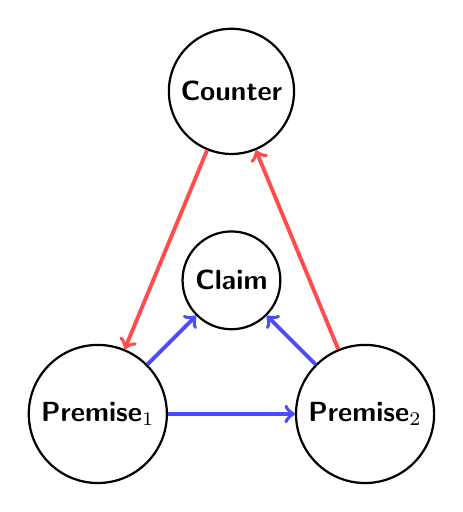
\begin{tikzpicture}[node distance=2.4cm]
        \tikzset{
            arg/.style={draw,circle,thick,minimum size=34pt,font=\sffamily\bfseries},
            support/.style={->, line width=1.4pt, color=blue!70},
            defeat/.style={->, line width=1.4pt, color=red!70}
        }
        \node[arg] (a) {Claim};
        \node[arg] (b) [below left of=a] {Premise$_1$};
        \node[arg] (c) [below right of=a] {Premise$_2$};
        \node[arg] (d) [above of=a] {Counter};
        \draw[support] (b) -- (a);
        \draw[support] (c) -- (a);
        \draw[support] (b) -- (c);
        \draw[defeat] (d) -- (b);
        \draw[defeat] (c) -- (d);
    \end{tikzpicture}
    \caption{Illustrative bipolar argumentation fragment with
             mutual support and derived defeat chains.}
    \label{fig:baf}
\end{figure}

\section{From Argumentation Mining to PASP}
\label{sec:contribution:pasp}

Argumentation mining systems extract structures such as
Figure~\ref{fig:baf} from text. Early joint models use Integer Linear
Programming to reconcile local classifiers with global constraints
\citep{stab2017parsing}. Probabilistic Logic Programming (PLP) broadens this
perspective: ProbLog enables uncertainty-aware reasoning while preserving
declarative structure \citep{fierens2015inference}. Deep learning can feed
probabilistic choices, as recent neuro-symbolic pipelines demonstrate
\citep{cerveira2023argumentation}.

Stable-model semantics further increase expressiveness. \textsc{smProbLog}
adopts PASP to handle negative cycles and sceptical reasoning that arise in
contradictory arguments \citep{totis2023smproblog}. The literature mostly
focuses on stratified programs for tractability, leaving the probabilistic
behaviour of non-stratified encodings largely unexplored. Our contribution is
to compile PASP representations of BAFs into structured circuits that support
efficient inference for both stratified and non-stratified cases, paving the way
for scalable neuro-symbolic training loops.

\section{Knowledge Compilation Pipeline}
\label{sec:contribution:pipeline}

Our pipeline grounds a PASP program obtained from a document, applies Clark’s
completion to expose a propositional theory, and then compiles the result into a
probabilistic circuit. Figure~\ref{fig:kc-pipeline} reuses the visual summary
from our poster to emphasise the offline--online separation: expensive
compilation happens once, while inference reuses the circuit.

\begin{figure}[ht]
    \centering
    \includegraphics[width=\linewidth]{slides/diagram.pdf}
    \caption{Knowledge compilation workflow for PASP argumentation programs.}
    \label{fig:kc-pipeline}
\end{figure}

The compilation stage must accommodate the probabilistic weights attached to
argumentative predicates and the loop formulas required by stable semantics
\citep{cozman2017semantics}. We use the 2AMC formalism to justify correctness
\citep{kiesel2022efficient} and adopt existing optimisations that control the
number of auxiliary variables introduced during completion
\citep{EITER2024104109}.

\section{Structured Circuits for Tractable Inference}
\label{sec:contribution:circuits}

The target circuits obey three structural properties that make weighted model
counting tractable \citep{Darwiche_2002, darwiche2011sdd}:
\begin{itemize}
    \item \textbf{Decomposability}: sub-circuits combined by a product node refer
          to disjoint sets of variables.
    \item \textbf{Determinism}: the children of a sum node are mutually
          exclusive, preventing double counting.
    \item \textbf{Smoothness}: the children of a sum node mention the same
          variables, enabling weight sharing and differentiation.
\end{itemize}

\begin{figure}[ht]
    \centering
    \begin{tikzpicture}[scale=1.05, every node/.style={font=\small}]
        \tikzset{
            sum/.style={draw,circle,thick,line width=1pt,inner sep=3pt,color=cyan!70!black},
            and/.style={draw,circle,thick,line width=1pt,inner sep=3pt,color=orange!80!black},
            lit/.style={font=\small\ttfamily}
        }
        \node[sum] (root) at (0,0) {$+$};
        \node[and] (and1) at (-2,-1.6) {$\times$};
        \node[and] (and2) at (2,-1.6) {$\times$};
        \node[sum] (sum1) at (-3.4,-3.2) {$+$};
        \node[lit] (litb) at (-0.6,-3.2) {$b$};
        \node[lit] (lita) at (-4.5,-4.8) {$a$};
        \node[lit] (litna) at (-2.3,-4.8) {$\neg a$};
        \node[lit] (litc) at (1.2,-3.2) {$a$};
        \node[lit] (litnb) at (3.0,-3.2) {$\neg b$};
        \draw (root) -- (and1);
        \draw (root) -- (and2);
        \draw (and1) -- (sum1);
        \draw (and1) -- (litb);
        \draw (sum1) -- (lita);
        \draw (sum1) -- (litna);
        \draw (and2) -- (litc);
        \draw (and2) -- (litnb);
    \end{tikzpicture}
    \caption{Smooth, decomposable, and deterministic circuit fragment used for
             PASP inference.}
    \label{fig:structured-circuit}
\end{figure}

Figure~\ref{fig:structured-circuit} highlights how the properties arise in
practice: the left branch considers two mutually exclusive cases for $a$ before
combining them with evidence about $b$, while the right branch enforces a
complementary scenario. These circuits support linear-time evaluation for
evidence updates and can be differentiated to align neural predictions with the
logical structure.

\section{Bottom-up Compilation via Apply}
\label{sec:contribution:bottom-up}

Our implementation follows the bottom-up philosophy of ASPMC and ProbLog
compilation \citep{vlasselaer2014compiling, vlasselaer2016tp}. Rather than
translating the entire completion into a CNF before compilation, we incrementally
construct circuits by conjoining and disjoining smaller blocks using the
\texttt{apply} operator of decision diagrams. This approach naturally extends
classic Binary Decision Diagrams (BDDs) \citep{bryant1986graph} to Sentential
Decision Diagrams (SDDs) \citep{darwiche2011sdd}, providing a more succinct
representation while preserving canonicity.

\begin{figure}[ht]
    \centering
    \includegraphics[width=.78\linewidth]{sdd_apply.pdf}
    \caption{Applying bottom-up compilation to merge local PASP fragments into
             a single structured circuit.}
    \label{fig:apply}
\end{figure}

Figure~\ref{fig:apply} illustrates how individual rule bodies are compiled and
merged. Each application of \texttt{apply} preserves the structural guarantees
of Figure~\ref{fig:structured-circuit}, allowing us to reuse partial results
whenever similar sub-programs appear across documents.

When Clark’s completion does introduce auxiliary variables, we rely on the
treewidth-aware strategies proposed by \citet{EITER2024104109} to keep the
resulting circuits compact. This bottom-up pipeline complements existing
top-down compilers, which remain the state of the art for large tractable PASP
instances but often struggle with the repeated updates required in
neuro-symbolic learning \citep{kiesel2022efficient}.

\section{Planned Experimental Analysis}
\label{sec:contribution:experiments}

Our empirical study will compare the scalability of the compiled circuits under
two settings: (i) stratified PASP programs that correspond to existing
neuro-symbolic pipelines, and (ii) non-stratified programs that capture richer
argumentative phenomena absent from current datasets. The core research
questions are therefore twofold:
\begin{itemize}
    \item How well do established knowledge-compilation techniques scale when
          applied to stratified argumentation programs extracted from text?
    \item Can the same techniques support non-stratified PASP encodings without
          sacrificing tractability, enabling novel neuro-symbolic models?
\end{itemize}

We leave dedicated space in this chapter to report the experimental findings,
ablation studies, and error analyses once the neuro-symbolic pipeline is fully
implemented.
